\documentclass[12pt,a4paper]{article}
\usepackage[utf8]{vietnam}
\usepackage{amsmath,amssymb}
\usepackage{tabularx}
\usepackage{tikz}
\usetikzlibrary{calc,angles,quotes,arrows.meta,patterns}
\usepackage{xcolor}
\usepackage{enumitem}
\usepackage{fancyhdr}
\usepackage{graphicx}
\usepackage[top=0.9cm, bottom=0.9cm, left=1.2cm, right=1.2cm]{geometry}
\usepackage[loigiai]{ex_test}
\SAOPTN{widthSA=3.2,heightSA=0.62}

\setlength{\headheight}{15pt}
\setlength{\parskip}{0pt}

\pagestyle{fancy}
\fancyhf{}
\rhead{\textit{Môn Toán 8 -- Hướng dẫn giải Đề số 07}}
\lhead{\textit{Bộ đề ôn tập Giữa học kì I}}
\cfoot{\thepage}

\begin{document}

\begin{center}
  \textbf{\Large HƯỚNG DẪN GIẢI CHI TIẾT VÀ BẢNG ĐÁP ÁN}\\
  \textbf{\large ĐỀ ÔN TẬP GIỮA HỌC KỲ I -- ĐỀ SỐ 07}\\
  \textit{Môn: Toán 8 -- Năm học 2026 -- 2027}
\end{center}
\vspace{2mm}

% --- BẢNG ĐÁP ÁN TRẮC NGHIỆM TÓM TẮT ---
\noindent\textbf{\large A. BẢNG ĐÁP ÁN TRẮC NGHIỆM TỔNG HỢP}
\vspace{1mm}

\noindent\textbf{1. Phần I (Mỗi câu trả lời đúng được 0,25 điểm):}
\begin{center}
\begin{tabular}{|c|c|c|c|c|c|c|c|c|c|c|c|c|}
\hline
\textbf{Câu} & \textbf{1} & \textbf{2} & \textbf{3} & \textbf{4} & \textbf{5} & \textbf{6} & \textbf{7} & \textbf{8} & \textbf{9} & \textbf{10} & \textbf{11} & \textbf{12} \\
\hline
\textbf{Đ/A} & \textbf{C} & \textbf{B} & \textbf{A} & \textbf{B} & \textbf{C} & \textbf{A} & \textbf{A} & \textbf{A} & \textbf{B} & \textbf{C} & \textbf{C} & \textbf{A} \\
\hline
\end{tabular}
\end{center}
\vspace{0.5mm}

\noindent\textbf{2. Phần II (Đúng 1 ý: 0,1đ; 2 ý: 0,25đ; 3 ý: 0,5đ; 4 ý: 1,0đ):}
\begin{center}
\begin{tabular}{|c|c|c|c|c||c|c|c|c|c|}
\hline
\textbf{Câu} & \textbf{a)} & \textbf{b)} & \textbf{c)} & \textbf{d)} & \textbf{Câu} & \textbf{a)} & \textbf{b)} & \textbf{c)} & \textbf{d)} \\
\hline
\textbf{Câu 1} & \textbf{Đ} & \textbf{Đ} & \textbf{Đ} & \textbf{S} & \textbf{Câu 2} & \textbf{Đ} & \textbf{Đ} & \textbf{Đ} & \textbf{S} \\
\hline
\end{tabular}
\end{center}
\vspace{0.5mm}

\noindent\textbf{3. Phần III (Mỗi câu trả lời đúng được 1,0 điểm):}
\begin{center}
\begin{tabular}{|c|c|c|}
\hline
\textbf{Câu} & \textbf{Câu 1} & \textbf{Câu 2} \\
\hline
\textbf{Đáp án} & $\mathbf{100}$ & $\mathbf{x = 0; x = 2; x = -2}$ \\
\hline
\end{tabular}
\end{center}
\vspace{1.5mm}

% --- B. LỜI GIẢI CHI TIẾT ---
\noindent\textbf{\large B. LỜI GIẢI CHI TIẾT CÁC CÂU HỎI}
\vspace{1mm}
\begin{ex}
Trong các biểu thức sau, biểu thức nào không phải là đơn thức?
\choice
{$-2xy^2$}
{$7$}
{\True $x + 2y$}
{$3xy$}
\loigiai{
Đơn thức là biểu thức chỉ gồm một số, một biến hoặc một tích giữa các số và biến. Biểu thức $x + 2y$ chứa phép cộng giữa các biến nên là đa thức, không phải là đơn thức.
}
\end{ex}

\begin{ex}
Cặp đơn thức nào sau đây là hai đơn thức đồng dạng?
\choice
{$2x^2y$ và $2xy^2$}
{\True $-3x^3y^2$ và $5x^3y^2$}
{$4x^2$ và $4x^3$}
{$2xy$ và $xy^2$}
\loigiai{
Hai đơn thức đồng dạng có hệ số khác 0 và có cùng phần biến. Hai đơn thức $-3x^3y^2$ và $5x^3y^2$ có cùng phần biến là $x^3y^2$.
}
\end{ex}

\begin{ex}
Bậc của đa thức $Q = x^2y^4 - 3x^5y + 2x^2y - 5$ là:
\choice
{\True 6}
{5}
{4}
{3}
\loigiai{
Hạng tử $x^2y^4$ có bậc là $2 + 4 = 6$; hạng tử $-3x^5y$ có bậc là $5 + 1 = 6$; hạng tử $2x^2y$ có bậc là $2 + 1 = 3$. Bậc của đa thức là bậc của hạng tử có bậc cao nhất, do đó bậc của $Q$ bằng 6.
}
\end{ex}

\begin{ex}
Kết quả của phép nhân $-3x^2 \cdot (2x - y)$ là:
\choice
{$-6x^3 - 3x^2y$}
{\True $-6x^3 + 3x^2y$}
{$-6x^2 + 3x^2y$}
{$6x^3 - 3x^2y$}
\loigiai{
Thực hiện phép nhân đơn thức với đa thức: $-3x^2 \cdot 2x - (-3x^2) \cdot y = -6x^3 + 3x^2y$.
}
\end{ex}

\begin{ex}
Biểu thức $x^2 - 4y^2$ được viết dưới dạng tích là:
\choice
{$(x - 2y)^2$}
{$(x - 4y)(x + 4y)$}
{\True $(x - 2y)(x + 2y)$}
{$(x + 2y)^2$}
\loigiai{
Áp dụng hằng đẳng thức hiệu hai bình phương: $x^2 - 4y^2 = x^2 - (2y)^2 = (x - 2y)(x + 2y)$.
}
\end{ex}

\begin{ex}
Đa thức $x^2 - 6x + 9$ được viết dưới dạng bình phương của một hiệu là:
\choice
{\True $(x - 3)^2$}
{$(x + 3)^2$}
{$(x - 9)^2$}
{$(x + 9)^2$}
\loigiai{
Áp dụng hằng đẳng thức bình phương của một hiệu: $x^2 - 6x + 9 = x^2 - 2 \cdot x \cdot 3 + 3^2 = (x - 3)^2$.
}
\end{ex}

\begin{ex}
Kết quả của phép tính $(-15x^3y^4) : (3xy^2)$ là:
\choice
{\True $-5x^2y^2$}
{$5x^2y^2$}
{$-5x^4y^6$}
{$-5x^2y$}
\loigiai{
Chia hệ số cho hệ số và chia phần biến cho phần biến: $(-15 : 3)(x^3 : x)(y^4 : y^2) = -5x^2y^2$.
}
\end{ex}

\begin{ex}
Cho tứ giác $EFGH$ có $\widehat{E} = 70^\circ$, $\widehat{F} = 110^\circ$, $\widehat{G} = 80^\circ$. Số đo góc $H$ là:
\choice
{\True $100^\circ$}
{$90^\circ$}
{$80^\circ$}
{$110^\circ$}
\loigiai{
Tổng các góc trong một tứ giác bằng $360^\circ$. Do đó: $\widehat{H} = 360^\circ - (70^\circ + 110^\circ + 80^\circ) = 360^\circ - 260^\circ = 100^\circ$.
}
\end{ex}

\begin{ex}
Tứ giác có các cạnh đối song song là:
\choice
{Hình thang}
{\True Hình bình hành}
{Hình chữ nhật}
{Hình thoi}
\loigiai{
Theo định nghĩa, hình bình hành là tứ giác có các cạnh đối song song.
}
\end{ex}

\begin{ex}
Hình bình hành có hai đường chéo vuông góc với nhau là:
\choice
{Hình chữ nhật}
{Hình thang cân}
{\True Hình thoi}
{Hình vuông}
\loigiai{
Theo dấu hiệu nhận biết, hình bình hành có hai đường chéo vuông góc với nhau là hình thoi.
}
\end{ex}

\begin{ex}
Mặt đáy của hình chóp tam giác đều là hình gì?
\choice
{Tam giác cân}
{Tam giác vuông}
{\True Tam giác đều}
{Tam giác vuông cân}
\loigiai{
Theo định nghĩa hình chóp tam giác đều, mặt đáy của hình chóp là một tam giác đều.
}
\end{ex}

\begin{ex}
Cho hình chóp tam giác đều có độ dài cạnh đáy bằng $4\text{ cm}$ và độ dài trung đoạn bằng $9\text{ cm}$. Diện tích xung quanh của hình chóp đó là:
\choice
{\True $54\text{ cm}^2$}
{$108\text{ cm}^2$}
{$36\text{ cm}^2$}
{$27\text{ cm}^2$}
\loigiai{
Chu vi đáy của hình chóp tam giác đều: $C = 3 \cdot 4 = 12\text{ cm}$. Diện tích xung quanh: $S_{xq} = \dfrac{1}{2} C \cdot d = \dfrac{1}{2} \cdot 12 \cdot 9 = 54\text{ cm}^2$.
}
\end{ex}


\setcounter{ex}{0}
\noindent\textbf{\large PHẦN II. CÂU TRẮC NGHIỆM ĐÚNG SAI}
\vspace{1mm}
\begin{ex}
Cho biểu thức $A = \left(\dfrac{x}{x^2 - 4} + \dfrac{1}{x + 2}\right) : \dfrac{2}{x - 2}$ với $x \neq \pm 2$. Xét tính đúng sai của các mệnh đề sau:
\choiceTF
{\True Mẫu thức chung của hai phân thức trong ngoặc là $x^2 - 4$}
{\True Kết quả rút gọn biểu thức trong ngoặc là $\dfrac{2x - 2}{x^2 - 4}$}
{\True Kết quả rút gọn của biểu thức $A$ là $\dfrac{x - 1}{x + 2}$}
{Có đúng 2 giá trị nguyên của $x$ để biểu thức $A$ nhận giá trị nguyên}
\loigiai{
\textbf{a)} \textbf{Đúng.} Mẫu thức chung là $(x - 2)(x + 2) = x^2 - 4$.

\textbf{b)} \textbf{Đúng.} Ta có: $\dfrac{x}{x^2 - 4} + \dfrac{x - 2}{x^2 - 4} = \dfrac{2x - 2}{x^2 - 4}$.

\textbf{c)} \textbf{Đúng.} $A = \dfrac{2(x - 1)}{(x - 2)(x + 2)} \cdot \dfrac{x - 2}{2} = \dfrac{x - 1}{x + 2}$.

\textbf{d)} \textbf{Sai.} Ta có $A = \dfrac{x + 2 - 3}{x + 2} = 1 - \dfrac{3}{x + 2}$. Để $A$ nguyên thì $x + 2 \in \{\pm 1; \pm 3\} \Rightarrow x \in \{-1; -3; 1; -5\}$ (gồm 4 giá trị nguyên thỏa mãn $x \neq \pm 2$).
}
\end{ex}

\begin{ex}
Hàm số bậc nhất $y = (m - 1)x + 2m - 3$ (với $m \neq 1$) có đồ thị là đường thẳng $(d)$. Xét tính đúng sai của các mệnh đề sau:
\choiceTF
{\True Với $m = 2$, hàm số đồng biến trên $\mathbb{R}$}
{\True Với $m = 0$, đồ thị $(d)$ đi qua điểm $A(1; -4)$}
{\True Đường thẳng $(d)$ song song với đường thẳng $y = 2x + 1$ khi $m = 3$}
{Khoảng cách từ gốc tọa độ $O$ đến đường thẳng $(d)$ khi $m = 2$ bằng $\sqrt{5}$}
\loigiai{
\textbf{a)} \textbf{Đúng.} Khi $m = 2$, hệ số $a = 2 - 1 = 1 > 0$ nên hàm số đồng biến trên $\mathbb{R}$.

\textbf{b)} \textbf{Đúng.} Khi $m = 0$, hàm số là $y = -x - 3$. Thay $x = 1 \Rightarrow y = -4$, nên đồ thị đi qua $A(1; -4)$.

\textbf{c)} \textbf{Đúng.} Đường thẳng $(d)$ song song với $y = 2x + 1$ khi $m - 1 = 2 \Leftrightarrow m = 3$ và $2m - 3 = 3 \neq 1$ (thỏa mãn).

\textbf{d)} \textbf{Sai.} Khi $m = 2$, đường thẳng là $x - y + 1 = 0$. Khoảng cách từ $O(0;0)$ đến $(d)$ là $d = \dfrac{|1|}{\sqrt{1^2 + (-1)^2}} = \dfrac{\sqrt{2}}{2} \neq \sqrt{5}$.
}
\end{ex}


\setcounter{ex}{0}
\noindent\textbf{\large PHẦN III. CÂU HỎI TRẢ LỜI NGẮN}
\vspace{1mm}
\begin{ex}
Tính giá trị của biểu thức $A = (x + 2y)^2 - (x - 2y)^2$ tại $x = 25$ và $y = \dfrac{1}{2}$. \shortans{100}
\loigiai{
Khai triển và thu gọn biểu thức $A$:

$A = (x^2 + 4xy + 4y^2) - (x^2 - 4xy + 4y^2) = 8xy$.

Thay $x = 25$ và $y = \dfrac{1}{2}$ vào biểu thức, ta được: $A = 8 \cdot 25 \cdot \dfrac{1}{2} = 100$.
}
\end{ex}

\begin{ex}
Tìm các giá trị của $x$, biết: $x^3 - 4x = 0$. \shortans{$x = 0; x = 2; x = -2$}
\loigiai{
Phân tích vế trái thành nhân tử:

$x(x^2 - 4) = 0 \Leftrightarrow x(x - 2)(x + 2) = 0$.

Suy ra $x = 0$ hoặc $x = 2$ hoặc $x = -2$.
}
\end{ex}


\setcounter{ex}{0}
\noindent\textbf{\large PHẦN IV. TỰ LUẬN (HƯỚNG DẪN GIẢI VÀ THANG ĐIỂM)}
\vspace{1mm}
\begin{ex} (1,0 điểm)
Rút gọn các biểu thức sau:
\begin{enumerate}[label=\textbf{\alph*)}, leftmargin=0.8cm, itemsep=0pt, topsep=1pt]
\item (0,35 điểm) $3x(2xy - 5) - 6x^2y$
\item (0,35 điểm) $(3x^4y^4 - 9x^2y^2 + 15xy^3) : (xy^2)$
\item (0,3 điểm) $(x - 3)^2 - (x + 3)^2$
\end{enumerate}
\loigiai{
\textbf{a)} \textit (0,35 điểm): $3x(2xy - 5) - 6x^2y = 6x^2y - 15x - 6x^2y = -15x$.

\textbf{b)} \textit (0,35 điểm): $(3x^4y^4 - 9x^2y^2 + 15xy^3) : (xy^2) = 3x^4y^4 : xy^2 - 9x^2y^2 : xy^2 + 15xy^3 : xy^2 = 3x^3y^2 - 9x + 15y$.

\textbf{c)} \textit (0,3 điểm): $(x - 3)^2 - (x + 3)^2 = (x^2 - 6x + 9) - (x^2 + 6x + 9) = -12x$.


}
\end{ex}
\vspace{0.5mm}

\begin{ex} (0,75 điểm)
Tìm $x$, biết:
\begin{enumerate}[label=\textbf{\alph*)}, leftmargin=0.8cm, itemsep=0pt, topsep=1pt]
\item (0,25 điểm) $2x(x - 5) - 2x^2 = 20$
\item (0,25 điểm) $(x + 3)^2 - x(x - 2) = 11$
\item (0,25 điểm) $x^2 - 9 + (x - 3)(2x + 1) = 0$
\end{enumerate}
\loigiai{
\textbf{a)} \textit (0,25 điểm): $2x(x - 5) - 2x^2 = 20 \Leftrightarrow 2x^2 - 10x - 2x^2 = 20 \Leftrightarrow -10x = 20 \Leftrightarrow x = -2$.

\textbf{b)} \textit (0,25 điểm): $(x + 3)^2 - x(x - 2) = 11 \Leftrightarrow x^2 + 6x + 9 - x^2 + 2x = 11 \Leftrightarrow 8x + 9 = 11 \Leftrightarrow 8x = 2 \Leftrightarrow x = \dfrac{1}{4}$.

\textbf{c)} \textit (0,25 điểm): $x^2 - 9 + (x - 3)(2x + 1) = 0 \Leftrightarrow (x - 3)(x + 3) + (x - 3)(2x + 1) = 0 \Leftrightarrow (x - 3)[(x + 3) + (2x + 1)] = 0 \Leftrightarrow (x - 3)(3x + 4) = 0 \Leftrightarrow x = 3$ hoặc $x = -\dfrac{4}{3}$.


}
\end{ex}
\vspace{0.5mm}

\begin{ex} (0,75 điểm)
Do ảnh hưởng của một cơn bão, một cây cột điện có phương thẳng đứng đã bị gió bão làm gãy ngang thân (như hình vẽ bên dưới), ngọn cây cột điện chạm đất cách gốc $4\text{ m}$, chiều cao từ gốc cây cột điện đến điểm gãy là $3\text{ m}$. Tính chiều cao ban đầu của cây cột điện.
\begin{center}
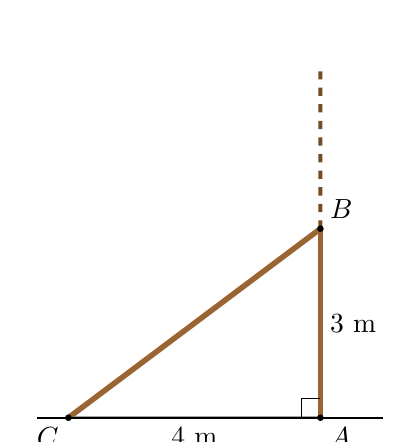
\begin{tikzpicture}[scale=0.8, >=stealth]
  \coordinate (A) at (4,0);
  \coordinate (C) at (0,0);
  \coordinate (B) at (4,3);
  \draw[thick] (C)--(A)--(B)--cycle;
  \draw[dashed, brown!60!black, line width=1.5pt] (B)--(4,5.5);
  \draw[line width=2pt, brown!80!black] (A)--(B);
  \draw[line width=2pt, brown!80!black] (B)--(C);
  \draw[thick] (-0.5,0)--(5,0);
  \fill (A) circle (1.5pt) node[below right] {$A$};
  \fill (B) circle (1.5pt) node[above right] {$B$};
  \fill (C) circle (1.5pt) node[below left] {$C$};
  \draw (3.7,0) |- (4,0.3);
  \node[right] at ($(A)!0.5!(B)$) {$3\text{ m}$};
  \node[below] at ($(A)!0.5!(C)$) {$4\text{ m}$};
\end{tikzpicture}
\end{center}
\begin{enumerate}[label=\textbf{\alph*)}, leftmargin=0.8cm, itemsep=0pt, topsep=1pt]
\item (0,75 điểm) Tính chiều cao ban đầu của cây cột điện.
\end{enumerate}
\loigiai{
\textbf{a)} \textit (0,75 điểm): Mô hình hóa hình ảnh cây cột điện bị gãy bằng tam giác $ABC$ vuông tại $A$.

Trong đó $AB = 3\text{ m}$ là chiều cao từ gốc đến điểm gãy, $AC = 4\text{ m}$ là khoảng cách từ gốc đến ngọn chạm đất, $BC$ là độ dài đoạn cột điện bị gãy gập xuống.

Áp dụng định lý Pythagore trong tam giác vuông $ABC$:
$BC^2 = AB^2 + AC^2 = 3^2 + 4^2 = 9 + 16 = 25 \Rightarrow BC = 5\text{ m}$.

Chiều cao ban đầu của cây cột điện là: $AB + BC = 3 + 5 = 8\text{ m}$.


}
\end{ex}
\vspace{0.5mm}

\begin{ex} (0,5 điểm)
Tìm giá trị nhỏ nhất của biểu thức: $P = x^2 + 2y^2 - 2xy - 4y + 2026$.
\begin{enumerate}[label=\textbf{\alph*)}, leftmargin=0.8cm, itemsep=0pt, topsep=1pt]
\item (0,5 điểm) Tìm giá trị nhỏ nhất của $P$.
\end{enumerate}
\loigiai{
\textbf{a)} \textit (0,5 điểm): Biến đổi biểu thức $P$:

$P = (x^2 - 2xy + y^2) + (y^2 - 4y + 4) + 2022 = (x - y)^2 + (y - 2)^2 + 2022$.

Vì $(x - y)^2 \ge 0$ và $(y - 2)^2 \ge 0$ với mọi $x, y$, nên $P \ge 2022$ với mọi $x, y$.

Dấu "=" xảy ra khi và chỉ khi: $\begin{cases} y - 2 = 0 \\ x - y = 0 \end{cases} \Leftrightarrow x = y = 2$.

Vậy giá trị nhỏ nhất của $P$ là $2022$, đạt được khi $x = y = 2$.


}
\end{ex}
\vspace{0.5mm}


\enlargethispage{1.5cm}
\begin{center}
\rule{4cm}{0.4pt}\\
\textit{--- HẾT ---}
\end{center}
\end{document}
